%\VignetteIndexEntry{Scalable Bayesian inference for the inverse temperature of a hidden Potts model}
%\VignetteEngine{knitr::knitr}
%\VignetteKeyword{Approximate Bayesian Computation}
%\VignetteKeyword{Composite likelihood}
%\VignetteKeyword{Hidden Markov random field}
%\VignetteKeyword{Image analysis}
%\VignetteKeyword{Pseudo-marginal method}
%\VignetteKeyword{Thermodynamic integration}
\documentclass[nojss,shortnames]{jss}\usepackage[]{graphicx}\usepackage[]{color}
%% maxwidth is the original width if it is less than linewidth
%% otherwise use linewidth (to make sure the graphics do not exceed the margin)
\makeatletter
\def\maxwidth{ %
  \ifdim\Gin@nat@width>\linewidth
    \linewidth
  \else
    \Gin@nat@width
  \fi
}
\makeatother

\definecolor{fgcolor}{rgb}{0.345, 0.345, 0.345}
\newcommand{\hlnum}[1]{\textcolor[rgb]{0.686,0.059,0.569}{#1}}%
\newcommand{\hlstr}[1]{\textcolor[rgb]{0.192,0.494,0.8}{#1}}%
\newcommand{\hlcom}[1]{\textcolor[rgb]{0.678,0.584,0.686}{\textit{#1}}}%
\newcommand{\hlopt}[1]{\textcolor[rgb]{0,0,0}{#1}}%
\newcommand{\hlstd}[1]{\textcolor[rgb]{0.345,0.345,0.345}{#1}}%
\newcommand{\hlkwa}[1]{\textcolor[rgb]{0.161,0.373,0.58}{\textbf{#1}}}%
\newcommand{\hlkwb}[1]{\textcolor[rgb]{0.69,0.353,0.396}{#1}}%
\newcommand{\hlkwc}[1]{\textcolor[rgb]{0.333,0.667,0.333}{#1}}%
\newcommand{\hlkwd}[1]{\textcolor[rgb]{0.737,0.353,0.396}{\textbf{#1}}}%
\let\hlipl\hlkwb

\usepackage{framed}
\makeatletter
\newenvironment{kframe}{%
 \def\at@end@of@kframe{}%
 \ifinner\ifhmode%
  \def\at@end@of@kframe{\end{minipage}}%
  \begin{minipage}{\columnwidth}%
 \fi\fi%
 \def\FrameCommand##1{\hskip\@totalleftmargin \hskip-\fboxsep
 \colorbox{shadecolor}{##1}\hskip-\fboxsep
     % There is no \\@totalrightmargin, so:
     \hskip-\linewidth \hskip-\@totalleftmargin \hskip\columnwidth}%
 \MakeFramed {\advance\hsize-\width
   \@totalleftmargin\z@ \linewidth\hsize
   \@setminipage}}%
 {\par\unskip\endMakeFramed%
 \at@end@of@kframe}
\makeatother

\definecolor{shadecolor}{rgb}{.97, .97, .97}
\definecolor{messagecolor}{rgb}{0, 0, 0}
\definecolor{warningcolor}{rgb}{1, 0, 1}
\definecolor{errorcolor}{rgb}{1, 0, 0}
\newenvironment{knitrout}{}{} % an empty environment to be redefined in TeX

\usepackage{alltt}

%% need no \usepackage{Sweave.sty}
\usepackage{subcaption} % the subfigure and subfig packages are deprecated
\usepackage{amsmath}
\usepackage{amsfonts}
\usepackage{listings}

\newcounter{nalg} % defines algorithm counter
\renewcommand{\thenalg}{\arabic{nalg}} %defines appearance of the algorithm counter
\DeclareCaptionLabelFormat{algocaption}{Algorithm \thenalg} % defines a new caption label as Algorithm x.y

\lstnewenvironment{algorithm}[1][] %defines the algorithm listing environment
{   
    \refstepcounter{nalg} %increments algorithm number
    \captionsetup{labelformat=algocaption,labelsep=colon} %defines the caption setup for: it ises label format as the declared caption label above and makes label and caption text to be separated by a ':'
    \lstset{ %this is the stype
        mathescape=true,
        frame=tb,
        numbers=left, 
        escapeinside={(*@}{@*)},
        numberstyle=\small,
        keywordstyle=\color{black}\bfseries,
        keywords={input, output, return, datatype, function, if, else, foreach, while, begin, end, for, do, then, },
        xleftmargin=.04\textwidth,
        #1 % this is to add specific settings to an usage of this environment (for instnce, the caption and referable label)
    }
}
{}

\author{Matthew T. Moores\\University of Warwick \And
   Anthony N. Pettitt \And
   Kerrie Mengersen\\Queensland University of Technology}
\Plainauthor{MT Moores, AN Pettitt, K Mengersen}

\title{\proglang{R} Package \pkg{bayesImageS}: Bayesian Methods for Image Segmentation using a Hidden Potts Model}
\Plaintitle{R package bayesImageS: Bayesian Methods for Image Segmentation using a Hidden Potts Model}
\Shorttitle{R package bayesImageS}

\Abstract{
The inverse temperature parameter of the Potts model governs the strength of spatial cohesion and therefore has a substantial influence over the resulting model fit. A difficulty arises from the dependence of an intractable normalising constant on the value of this parameter and thus there is no closed form solution for sampling from the posterior distribution directly. There are a variety of computational approaches for sampling from the posterior without evaluating the normalising constant. These algorithms differ in their levels of accuracy and their scalability for datasets of realistic size.

This \proglang{R} package provides implementations of Markov chain Monte Carlo algorithms for sampling from the intractable posterior distribution of the Potts model. The algorithms include pseudolikelihood, the exchange algorithm, path sampling, and approximate Bayesian computation. The following vignette explains these algorithms, providing the necessary theoretical background as well as implementation details specific to our \proglang{R} package. We address important questions such as how the computational cost increases with the size of the images, as well as how much accuracy is lost by using faster, more approximate methods. This document is intended to provide guidance on selecting a suitable algorithm for Bayesian image analysis. For nontrivial images, this necessarily involves some degree of approximation to produce an acceptable compromise between accuracy and computational cost.}

\Keywords{approximate Bayesian computation, composite likelihood, hidden Markov random field, image analysis, pseudo-marginal method, thermodynamic integration}

\Address{
   Matthew T. Moores\\
   Department of Statistics\\
   University of Warwick\\
   Coventry CV4 7AL, United Kingdom\\
   E-mail: \email{M.T.Moores@warwick.ac.uk}\\
   URL: \url{http://warwick.ac.uk/mmoores}
}
\IfFileExists{upquote.sty}{\usepackage{upquote}}{}
\begin{document}

\section{Introduction}

Markov random field (MRF) models have seen widespread use in image analysis since their introduction by \citet{Besag1974}, as surveyed by \citet{Winkler2003} and \citet{Li2009}. A MRF is a generalisation of the Markovian dependence structure to more than one dimension: satellite imagery has two spatial dimensions, while medical images such as computed tomography (CT) are three-dimensional. The hidden \citet{Potts1952} model employs a latent MRF on discrete states to describe spatial dependence between adjacent neighbours. The degree of dependence in the model is governed by a parameter known as the inverse temperature due to its origin in statistical physics. It is difficult to set this parameter by trial and error, particularly for noisy images. Rather than using a fixed value, it would be preferable to estimate the inverse temperature as part of the model. However, the intractable normalising constant of the Potts model depends on the value of the inverse temperature, which means that there is no closed form solution for estimating its posterior distribution.

\citet{Ryden1998} derived a pseudolikelihood (PL) approximation \citep{Besag1975} to the intractable posterior density. \citet{Gelman1998} instead approximated the ratio of normalising constants using thermodynamic integration (TI), also known as path sampling. \citet{Moeller2006} introduced an auxiliary variable method that gives an exact MCMC algorithm for the special case of a 2 component Potts model, also known as an Ising model. \citet{Murray2006} proposed a variant of the exact method known as the exchange algorithm or multiple auxiliary variable method. By replacing the expensive perfect sampling step \citep{Propp1996} with an approximation such as Gibbs sampling, \citet{Cucala2009} developed an approximate exchange algorithm (AEA) that can be applied for Potts models with $k>2$. \citet{Friel2009} introduced the reduced dependence approximation (RDA) which uses recursion to calculate the normalising constant on small sub-lattices. \citet{McGrory2012} generalised RDA to an irregular lattice. \citet{Grelaud2009} used the sufficient statistic of the Potts model to estimate the inverse temperature using approximate Bayesian computation (ABC). \citet{Everitt2012} combined the approximate exchange algorithm with particle Markov chain Monte Carlo (PMCMC) and also implemented ABC with sequential Monte Carlo (SMC-ABC) for the Ising model. Although all of these methods work very well in theory, the largest image used in any of these papers to demonstrate an algorithm is less than ten thousand pixels. This does not give a reliable indication of how these algorithms might perform when applied to images of a more substantial size.


\section{Hidden Potts model}
\label{s:model}
Image segmentation can be viewed as the task of labelling the observed pixels $\mathbf{y}$ according to a finite set of discrete states $\mathbf{z} \in \{ 1, \dots, k \}$. The hidden Potts model allows for spatial correlation between neighbouring labels in the form of a Markov random field. The latent labels follow a Gibbs distribution, which is specified in terms of its conditional probabilities:
  \begin{equation}
  \label{eq:Potts}
  p(z_i | z_{\setminus i}, \beta) = \frac{\exp\left\{\beta\sum_{i \sim \ell}\delta(z_i,z_\ell)\right\}}{\sum_{j=1}^k \exp\left\{\beta\sum_{i \sim \ell}\delta(j,z_\ell)\right\}}
  \end{equation}
  where $\beta$ is the inverse temperature, $z_{\setminus i}$ represents all of the labels except $z_i$, $i \sim \ell$ are the  neighbouring pixels of $i$, and $\delta(u,v)$ is the Kronecker delta function. Thus, $\sum_{i \sim \ell}\delta(z_i,z_\ell)$ is a count of the neighbours that share the same label.

If the labels $z_i$ are indexed row-wise, the nearest (first-order) neighbours $i \sim \ell$ in a regular 2D lattice with $c$ columns are $\{ z_{i-1}, z_{i-c}, z_{i+c}, z_{i+1} \}$. Pixels situated at the boundary of the image domain have less than four neighbours. Likewise, voxels in a regular 3D lattice have a maximum of 6 first-order neighbours. These neighbourhood relationships are reciprocal, so $h \in i \sim \ell$ implies $i \in h \sim \ell$. If $\mathcal{E}$ is the set of all unique neighbour pairs, or edges in the image lattice, then $| \mathcal{E} | = 2(n - \sqrt{n})$ for a square lattice and $3(n - n^{2/3})$ for a cube.

The observation equation links the latent labels to the corresponding pixel values:
  \begin{equation}
  \label{eq:obs}
  p(\mathbf{y} | \mathbf{z}, \boldsymbol\theta) = \prod_{i=1}^n p(y_i | z_i, \theta_{z_i})
  \end{equation}
  where $\theta_{j}$ are the parameters that govern the distribution of the pixel values with label $j$. The hidden Potts model can thus be viewed as a spatially-correlated generalisation of the finite mixture model \citep{Ryden1998}. \citet{Green2002} used a Poisson likelihood for (\ref{eq:obs}), with intensity $\lambda_j$. Instead we follow \citet{Geman1984,Alston2007}, and many others in assuming that the pixels with label $j$ share a common mean $\mu_j$ corrupted by additive Gaussian noise with variance $\sigma_j^2$:
  \begin{equation}
  \label{eq:obs2}
y_i | z_i=j, \mu_j, \sigma^2_j \;\sim\; \mathcal{N}\left( \mu_j, \sigma^2_j \right)
  \end{equation}
 
The Gibbs distribution is a member of the exponential family and so there is a sufficient statistic for this model, as noted by \citet{Grelaud2009}:
  \begin{equation}
  \label{eq:potts_stat}
\mathrm{S}(\mathbf{z}) = \sum_{i \sim \ell \in \mathcal{E}} \delta(z_i,z_\ell)
  \end{equation}
This statistic represents the total number of like neighbour pairs in the image. The likelihood $p(\mathbf{y},\mathbf{z} | \boldsymbol\theta, \beta)$ can therefore be factorised into $p(\mathbf{y} | \mathbf{z}, \boldsymbol\theta) p(\mathrm{S}(\mathbf{z}) | \beta)$, where the second factor does not depend on the observed data, but only on the sufficient statistic. The joint posterior is then:
\begin{equation}
\label{eq:joint_post}
p(\boldsymbol\theta, \beta, \mathbf{z} | \mathbf{y}) \propto p(\mathbf{y} | \mathbf{z}, \boldsymbol\theta) \pi(\boldsymbol\theta) p(\mathrm{S}(\mathbf{z}) | \beta) \pi(\beta)
\end{equation}
The conditional distributions $p(\boldsymbol\theta | \mathbf{z}, \mathbf{y})$ and $p(z_i | z_{\setminus i}, \beta, y_i, \boldsymbol\theta_{z_i})$ can be simulated using Gibbs sampling, but $p(\beta | \mathbf{y}, \mathbf{z}, \boldsymbol\theta)$ involves an intractable normalising constant $\mathcal{C}(\beta)$:
  \begin{eqnarray}
  \label{eq:beta_post}
  p(\beta \mid \mathbf{y}, \mathbf{z}, \boldsymbol\theta) &\propto&  p(\mathrm{S}(\mathbf{z}) | \beta) \pi(\beta)\\
  \label{eq:beta}
 &\propto& \frac{\exp\left\{ \beta\, \mathrm{S}(\mathbf{z}) \right\}}{\mathcal{C}(\beta)} \pi(\beta)
  \end{eqnarray}
The normalising constant is also known as a partition function in statistical physics. It has computational complexity of $\mathcal{O}(n k^n)$, since it involves a sum over all possible combinations of the labels $\mathbf{z} \in \mathcal{Z}$:
  \begin{equation}
  \label{eq:norm}
\mathcal{C}(\beta) = \sum_{\mathbf{z} \in \mathcal{Z}} \exp\left\{\beta\, \mathrm{S}(\mathbf{z})\right\}
  \end{equation}
It is infeasible to calculate this value exactly for nontrivial images, thus computational approximations are required.
\begin{figure}
\centering
        \begin{subfigure}{0.45\textwidth}
                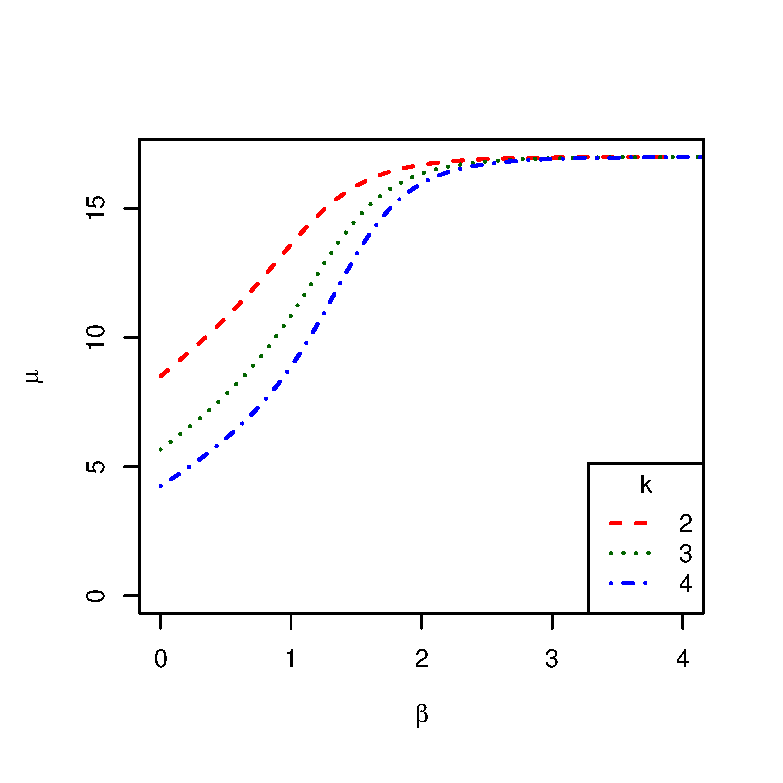
\includegraphics[width=\textwidth]{exact_exp_k.eps}
                \caption{Expectation for $n=12$ and increasing values of $k \in \{2, 3, 4\}$.}
                \label{f:exact_exp_k}
        \end{subfigure}
\qquad
        \begin{subfigure}{0.45\textwidth}
                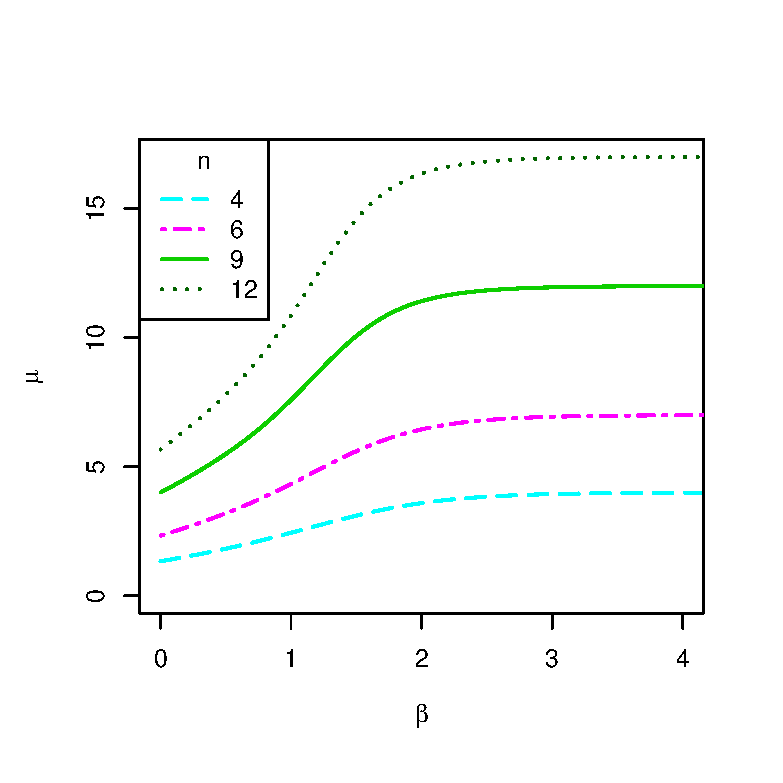
\includegraphics[width=\textwidth]{exact_exp_n.eps}
                \caption{Expectation for $k=3$ and increasing values of $n \in \{4, 6, 9, 12\}$.}
                \label{f:exact_exp_n}
        \end{subfigure}%
\qquad
        \begin{subfigure}{0.45\textwidth}
                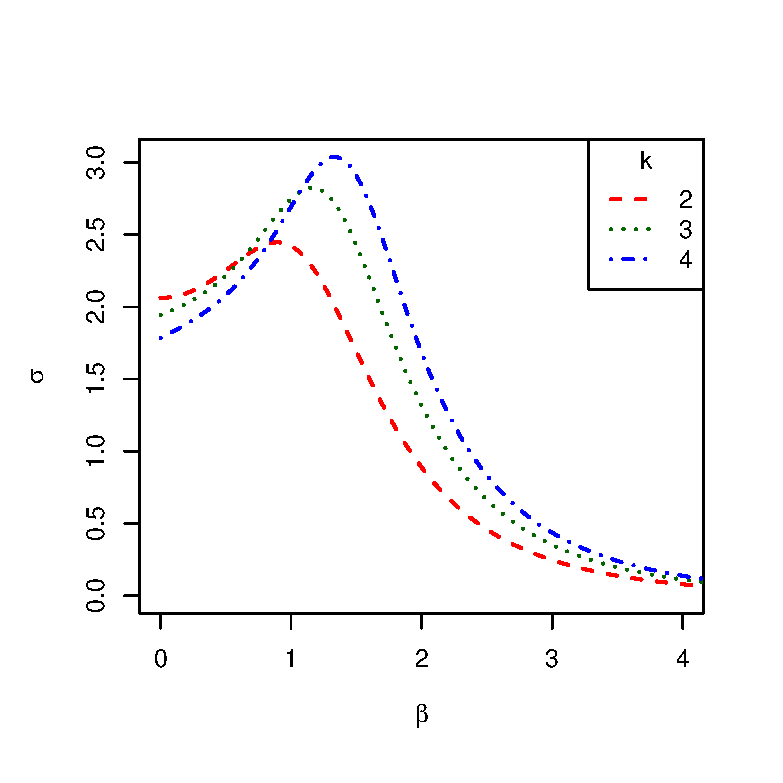
\includegraphics[width=\textwidth]{exact_var_k.eps}
                \caption{Standard deviation for $n=12$ and increasing values of $k \in \{2, 3, 4\}$.}
                \label{f:exact_var_k}
        \end{subfigure}%
\qquad
        \begin{subfigure}{0.45\textwidth}
                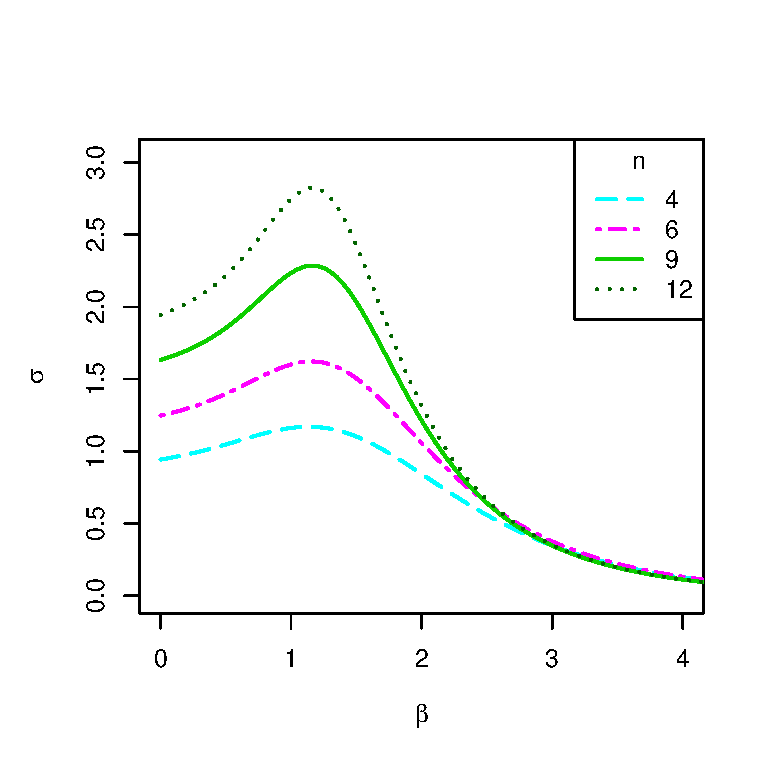
\includegraphics[width=\textwidth]{exact_var_n.eps}
                \caption{Standard deviation for $k=3$ and increasing values of $n \in \{4, 6, 9, 12\}$.}
                \label{f:exact_var_n}
        \end{subfigure}%
\caption[Distribution of the sufficient statistic of the Potts model]{Distribution of the sufficient statistic of the Potts model for increasing values of the inverse temperature $\beta$, the number of pixels $n$, and the number of unique labels $k$. The expectation and standard deviation of $\mathrm{S}(\mathbf{z})$ were calculated exactly, using a brute force method.}
\label{f:exact_beta}
\end{figure}

The conditional expectation of $\mathrm{S}(\mathbf{z})$ given $\beta$ can be expressed in terms of the normalising constant:
  \begin{equation}
  \label{eq:expSz}
\mathbb{E}_{\mathbf{z} | \beta}[\mathrm{S}(\mathbf{z})] = \frac{\mathrm d}{\mathrm d \beta} \log\{ \mathcal{C}(\beta) \}
  \end{equation}
 As $\beta$ approaches infinity, all of the pixels in the image are almost surely assigned the same label, thus the expectation of $\mathrm{S}(\mathbf{z})$ approaches the total number of edges $|\mathcal{E}|$ asymptotically, while the variance approaches zero. When $\beta = 0$, (\ref{eq:Potts}) simplifies to $\left(\sum_j \exp\{0\}\right)^{-1}$, hence the probability of any pair of neighbours being assigned the same label follows an independent Bernoulli distribution with $p = k^{-1}$. In this case, $\mathrm{S}(\mathbf{z})$ follows a Binomial distribution with expectation $|\mathcal{E}| /k$ and variance $|\mathcal{E}| k^{-1} (1 - k^{-1})$. In a finite image lattice the distribution of $\mathrm{S}(\mathbf{z})$ changes smoothly between these two extremes, as illustrated by Figure~\ref{f:exact_beta}, but its computation is intractable for nontrivial images.

The Potts model undergoes a phase transition at the critical value of $\beta$, switching from a disordered to an ordered state. \citet{Potts1952} showed that the critical value for a 2D lattice on a cylinder can be calculated exactly according to:
  \begin{equation}
  \label{eq:bcrit2d}
\beta_{crit} = \log\left\{1 + \sqrt{k}\right\}
  \end{equation}
The periodic boundary condition does not apply to the lattices considered in this paper, so for example the critical value for the images in Figure~\ref{f:exact_beta} is different to (\ref{eq:bcrit2d}). However, the error introduced by the finite boundary diminishes as $n$ increases. Figure~\ref{f:bcrit} shows that (\ref{eq:bcrit2d}) is very accurate in predicting the behaviour of $\mathrm{S}(\mathbf{z})$ for a 2D image with a maximum value of $\mathrm{S}(\mathbf{z})$ for first-order neighbours of 1,954,672, with k=6 mixture components and $\beta_{crit} \approx 1.24$. $\mathrm{S}(\mathbf{z})$ is approximated by simulation using the algorithm of \citet{Swendsen1987}. Figure~\ref{f:bcrit2d} shows that the gradient of the expectation becomes very steep near the critical region, which is reflected in the super-exponential increase of the standard deviation illustrated by Figure~\ref{f:bcrit2d_sd}. As $n \to \infty$ the derivative of the likelihood at the critical point, and hence the variance, is unbounded \citep{Pickard1987}. This heteroskedasticity has important implications for many of the methods discussed in Section~\ref{s:methods}. 
\begin{figure}
        \centering
        \begin{subfigure}{0.45\textwidth}
                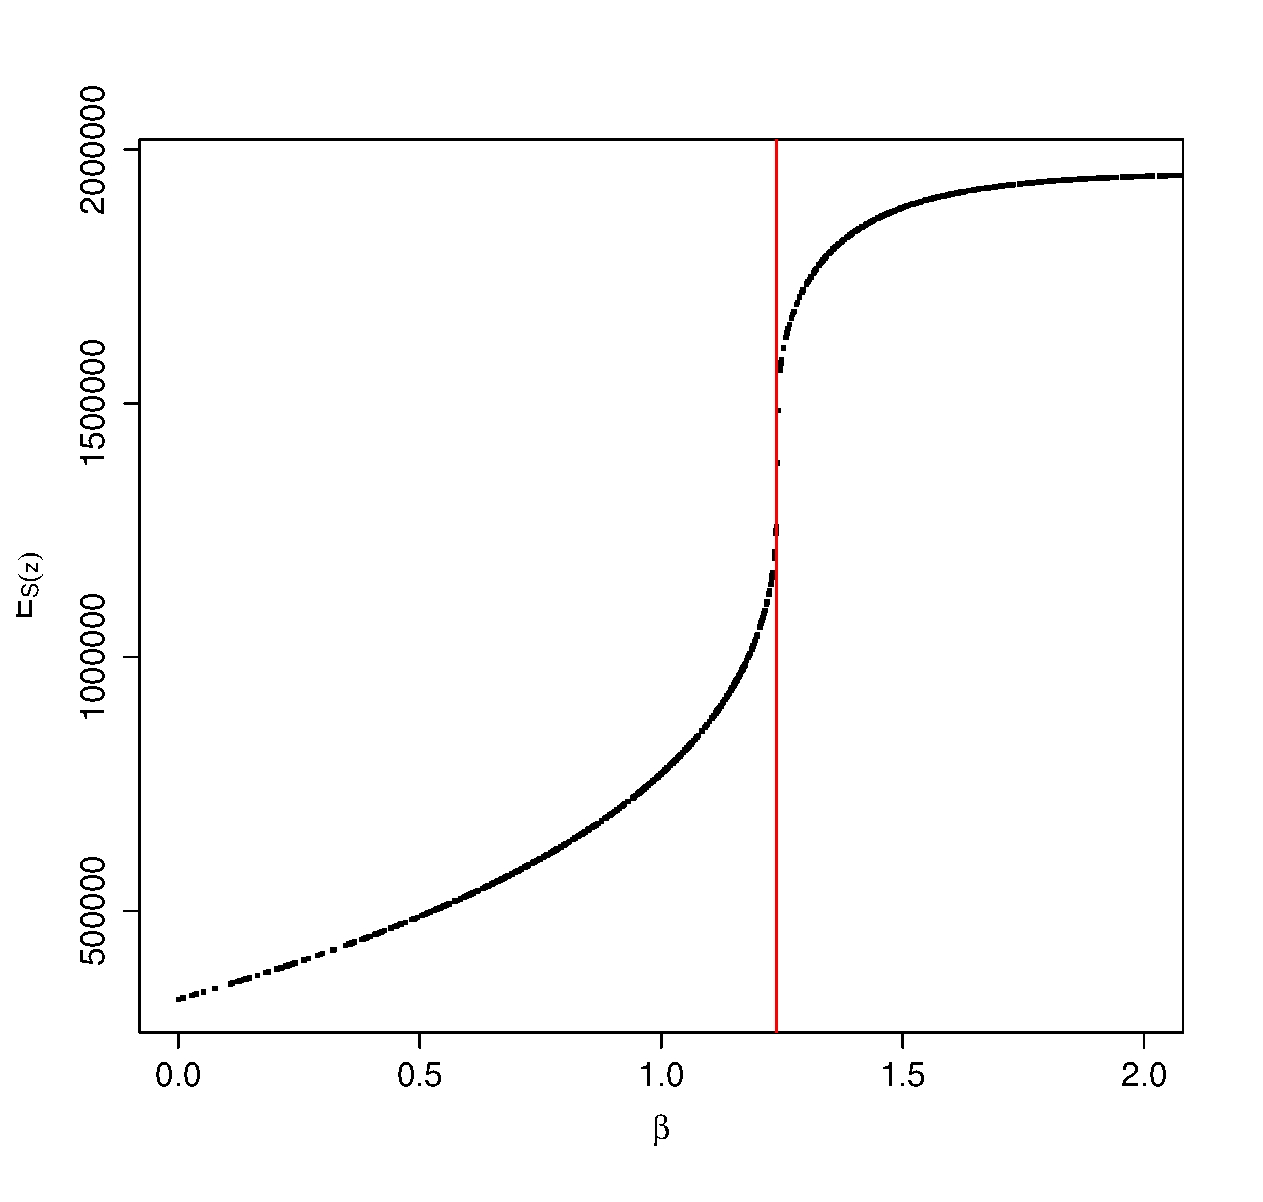
\includegraphics[width=\textwidth]{bcrit2d.eps}
                \caption{Expectation for a 2D Potts model with $k = 6$.}
                \label{f:bcrit2d}
        \end{subfigure}%
\qquad
        \begin{subfigure}{0.45\textwidth}
                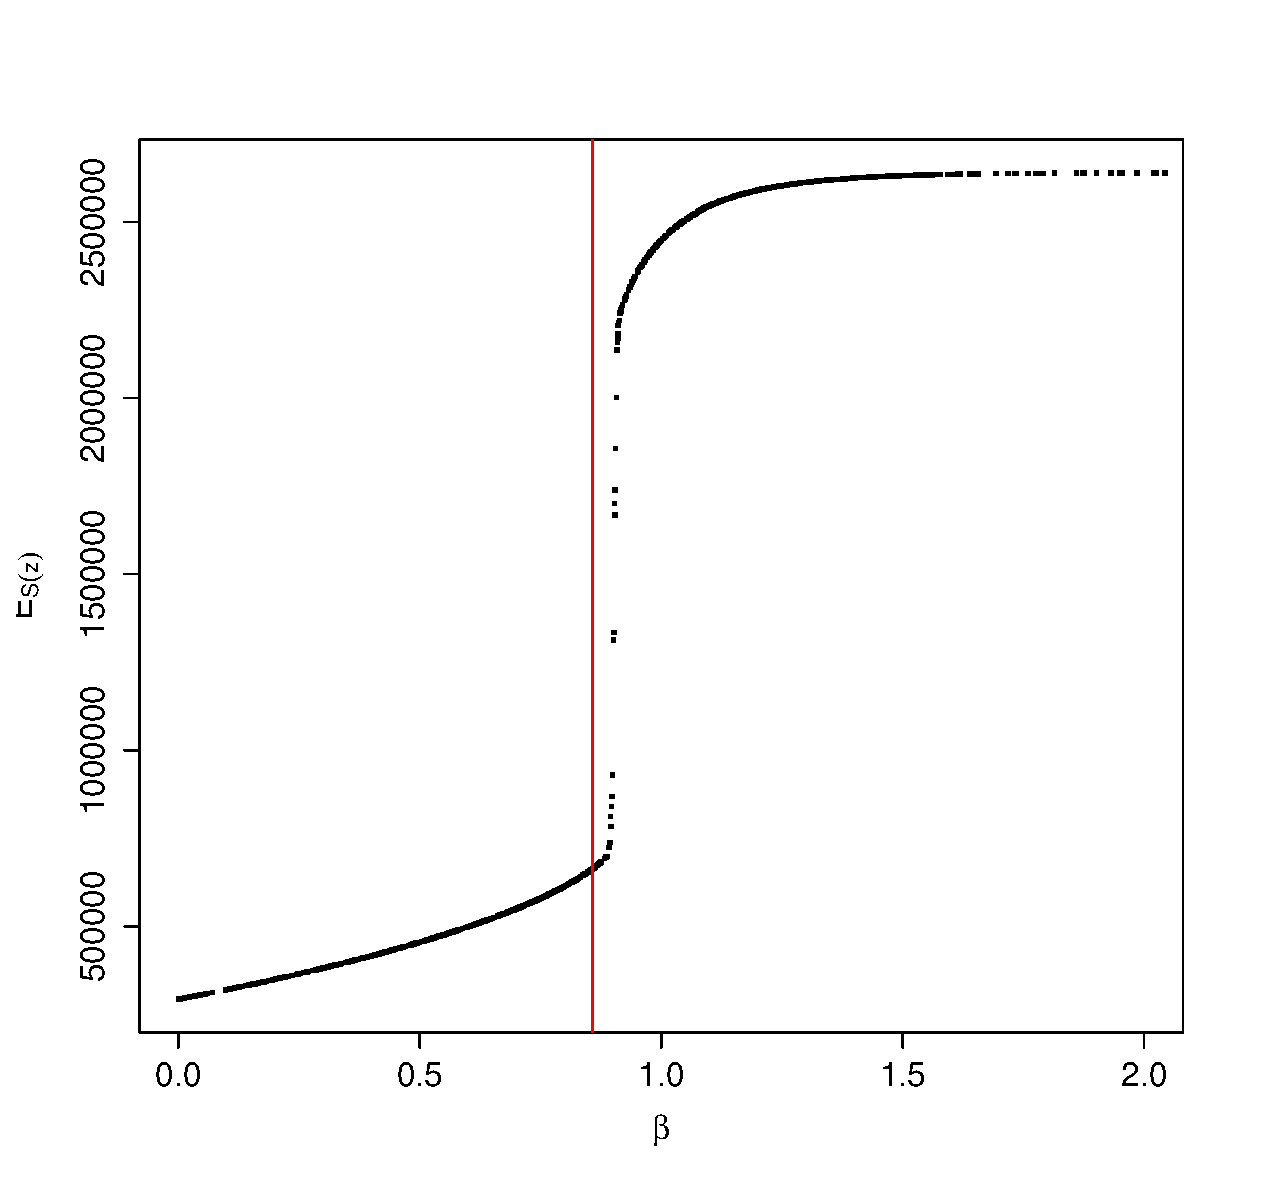
\includegraphics[width=\textwidth]{bcrit3d.eps}
                \caption{Expectation for a 3D Potts model with $k = 9$.}
                \label{f:bcrit3d}
        \end{subfigure}%
\qquad
        \begin{subfigure}{0.45\textwidth}
                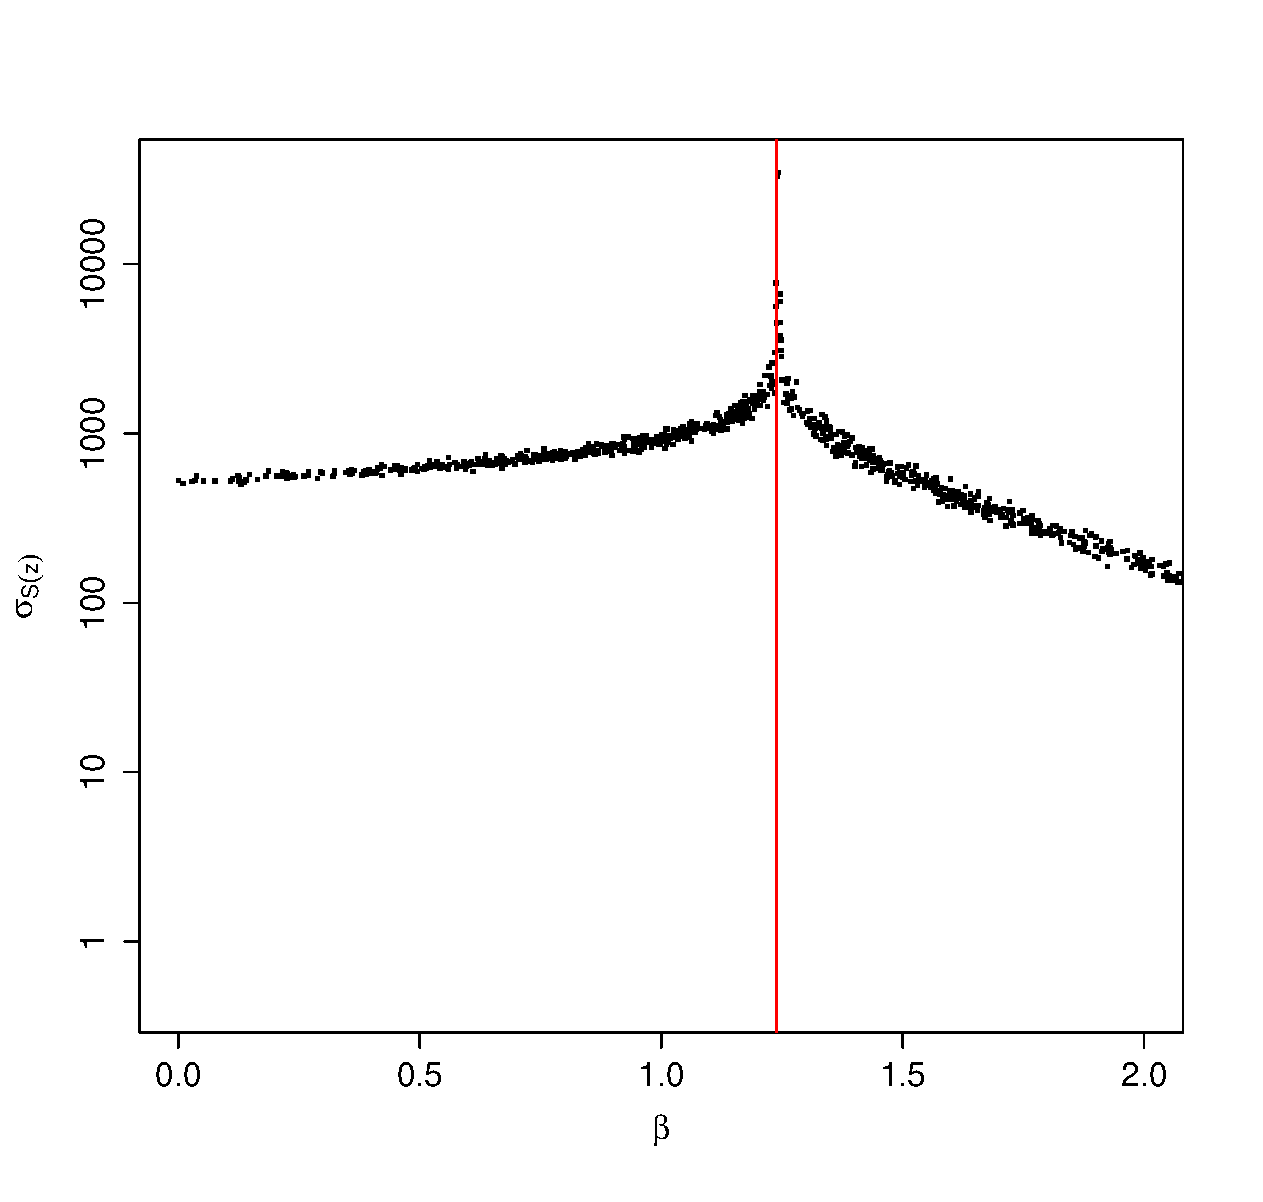
\includegraphics[width=\textwidth]{bcrit2d_sd.eps}
                \caption{Standard deviation for a 2D Potts model with $k = 6$.}
                \label{f:bcrit2d_sd}
        \end{subfigure}%
\qquad
        \begin{subfigure}{0.45\textwidth}
                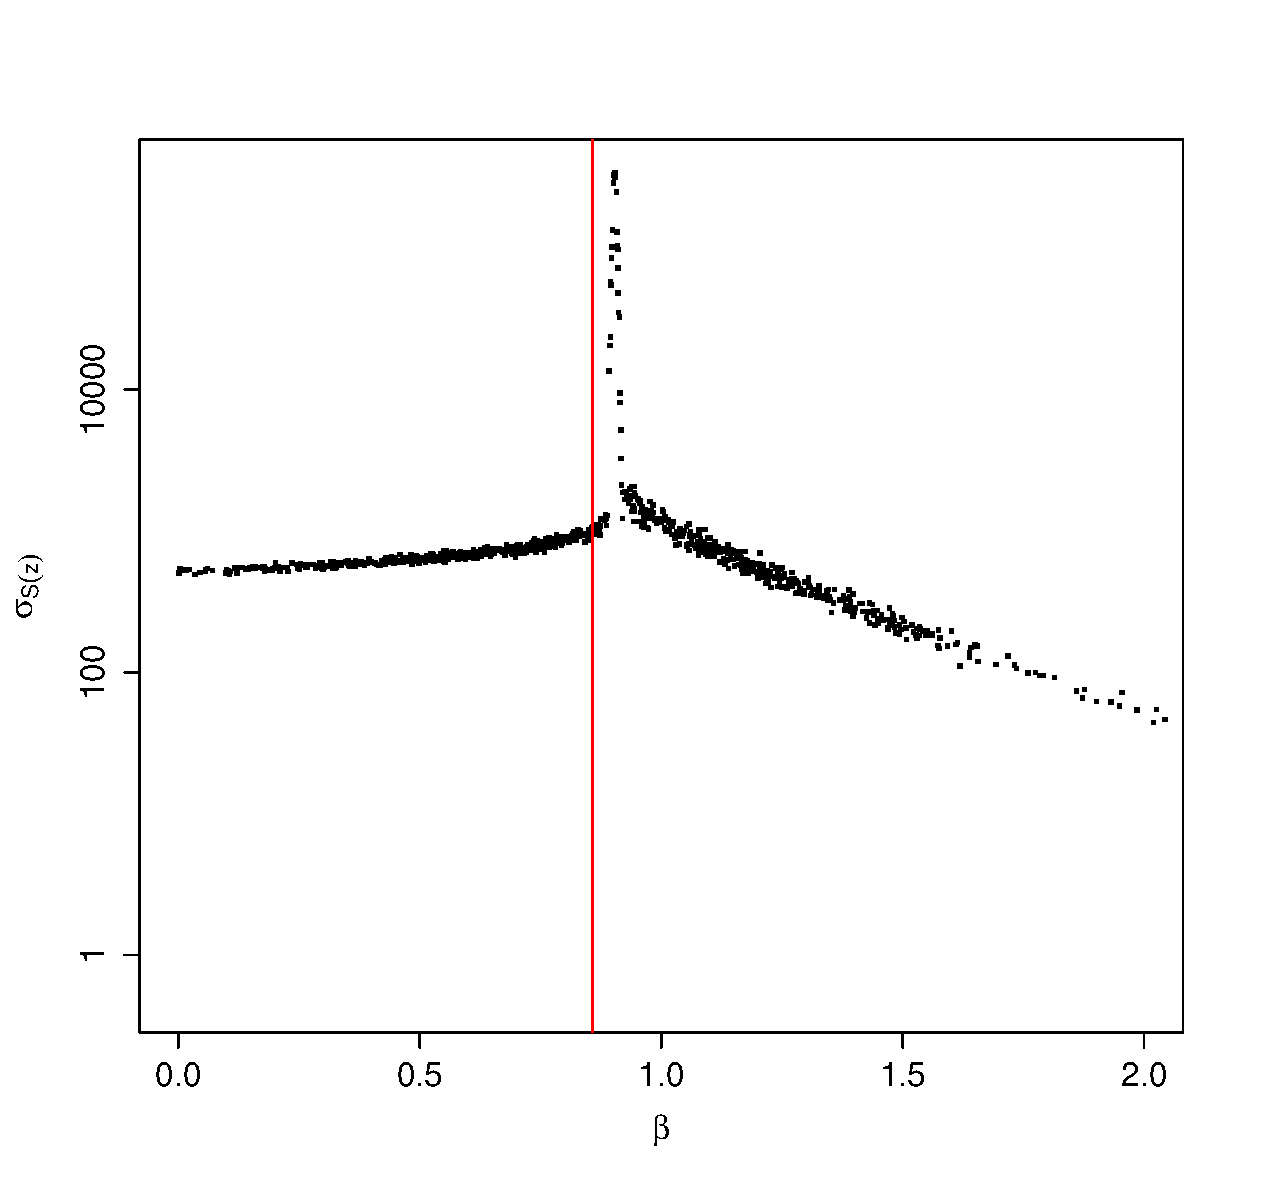
\includegraphics[width=\textwidth]{bcrit3d_sd.eps}
                \caption{Standard deviation for a 3D Potts model with $k = 9$.}
                \label{f:bcrit3d_sd}
        \end{subfigure}%
\caption{Approximate distribution of $\mathrm{S}(\mathbf{z})$ using Swendsen-Wang for a 2D image with $k=6$ and $|\mathcal{E}| \approx 2 \times 10^6$ (left) and a 3D image with $k=9$ and $|\mathcal{E}| \approx 3 \times 10^6$ (right). The vertical line is the critical value of $\beta$.}
\label{f:bcrit}
\end{figure}

There is no exact formula for $\beta_{crit}$ in 3D images, although \citet{Hajdukovic1983} developed an empirical approximation that works reasonably well:
  \begin{equation}
  \label{eq:bcrit3d}
\beta_{crit}  \approx \frac{2}{3} \log\left\{ \frac{1}{2} \left(\sqrt{2} + \sqrt{4k-2}\right) \right\}
  \end{equation}
The behaviour of $\mathbb{E}_{\mathbf{z} | \beta}[\mathrm{S}(\mathbf{z})]$ for a 3D image with $|\mathcal{E}|$ approximately equal to three million, $k=9$ and $\beta_{crit} \approx 0.86$ is illustrated by Figure~\ref{f:bcrit3d}. The standard deviation is shown in Figure~\ref{f:bcrit3d_sd}. It is evident that (\ref{eq:bcrit3d}) has underestimated $\beta_{crit}$ since the maximum value of the standard deviation occurs at $\beta = 0.9$.

\section{Computational methods}
\label{s:methods}
In this section we describe the four major algorithms for intractable likelihoods in Bayesian image analysis. These methods provide alternative means to simulate parameter values from (\ref{eq:beta}) without computing the normalising constant. We describe the algorithms in terms of Markov chain Monte Carlo (MCMC) to enable direct comparison, although we also mention other approaches where applicable, such as particle-based (SMC and PMCMC) methods. Reference implementations of all of these methods are available from various sources described below, but for the purpose of comparison we have reimplemented the algorithms using \pkg{RcppArmadillo} \citep{Eddelbuettel2013}.

\subsection{Pseudolikelihood and composite likelihood}
Pseudolikelihood is the simplest of the methods that we have considered and also the fastest. \citet{Ryden1998} showed that the intractable distribution (\ref{eq:beta}) could be approximated using the product of the conditional densities given by (\ref{eq:Potts}). This enables updates for the inverse temperature at iteration $t$ to be simulated using a Metropolis-Hastings (M-H) step, as shown in Algorithm~\ref{alg:pseudo}. 

\begin{algorithm}[float,caption={MCMC with pseudolikelihood (PL)}, label={alg:pseudo}]
Initialise $\beta_0, \boldsymbol\mu_0, \boldsymbol\sigma^2_0, \mathbf{z}_0$
for $t \in 1\dots T$ do
  Update the labels $z_i \sim p(y_i | z_i, \mu_{z_i}, \sigma^2_{z_i}) \,p(z_i | z_{\setminus i}, \beta) \; \forall i \in \{ 1, \dots, n\}$
  Calculate sufficient statistics $\bar{y}_j, s^2_j \; \forall z_i = j, \, \forall j \in \{ 1, \dots, k\}$
  Update the noise parameters $\mu_j, \sigma^2_j \sim p(\bar{y}_j, s^2_j | \mu_j, \sigma_j^2) \,\pi(\mu_j | \sigma^2_j) \, \pi(\sigma^2_j)$
  Draw proposed parameter value $\beta' \sim q(\beta' | \beta_{t-1})$
  Approximate $p(\mathbf{z}|\beta')$ and $p(\mathbf{z}|\beta_{t-1})$ using: (*@
 \begin{equation} \label{eq:pseudo}
p(\mathbf{z}|\beta) \approx \prod_{i=1}^n p(z_i | z_{\setminus i}, \beta)
\end{equation}  @*)
  Calculate the M-H ratio $\rho = \min\left( 1, \frac{p(\mathbf{z}|\beta') \pi(\beta') q(\beta_{t-1} | \beta')}{p(\mathbf{z}|\beta_{t-1}) \pi(\beta_{t-1}) q(\beta' | \beta_{t-1})} \right)$ (*@ \label{mh:ratio} @*)
  Draw $u \sim \mathrm{Uniform}[0,1]$
  if $u < \rho$ then (*@ \label{mh:accept} @*)
    $\beta_t \gets \beta'$ 
  else
    $\beta_t \gets \beta_{t-1}$ 
  end if
end for
\end{algorithm}

The M-H proposal density $q(\beta'|\beta_{t-1})$ can be any distribution such that $\int q(\beta'|\beta_{t-1})\, d\beta' = 1$. However, there is a tradeoff between exploring the full state space and ensuring that the probability of acceptance (at line~\ref{mh:accept}) is sufficiently high. We use the adaptive random walk (RWMH) algorithm of \citet{Garthwaite2010}, which automatically tunes the bandwidth of the proposal density to target a given M-H acceptance rate. When a symmetric proposal density is used, $q(\beta'|\beta_{t-1}) = q(\beta_{t-1}|\beta')$ and so this term cancels out in the M-H ratio on line~\ref{mh:ratio}. The natural logarithm of $\rho$ is used in practice to improve the numerical stability of Algorithm~\ref{alg:pseudo}. 

\begin{figure}
        \centering
        \begin{subfigure}{0.65\textwidth}
                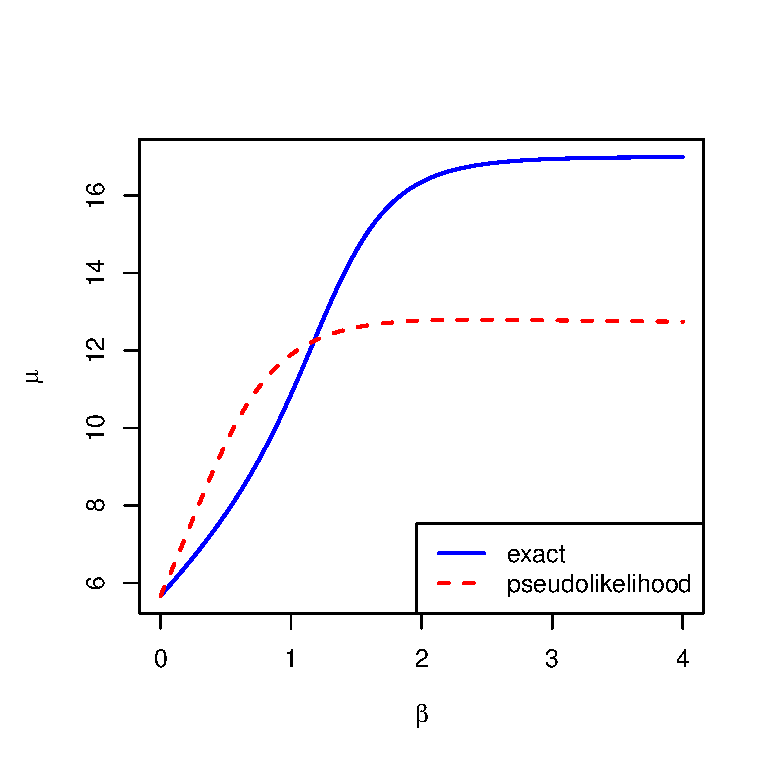
\includegraphics[width=\textwidth]{pl_exp_n12k3.eps}
                \caption{Expectation.}
                \label{f:pl_exp}
        \end{subfigure}%
\qquad
        \begin{subfigure}{0.65\textwidth}
                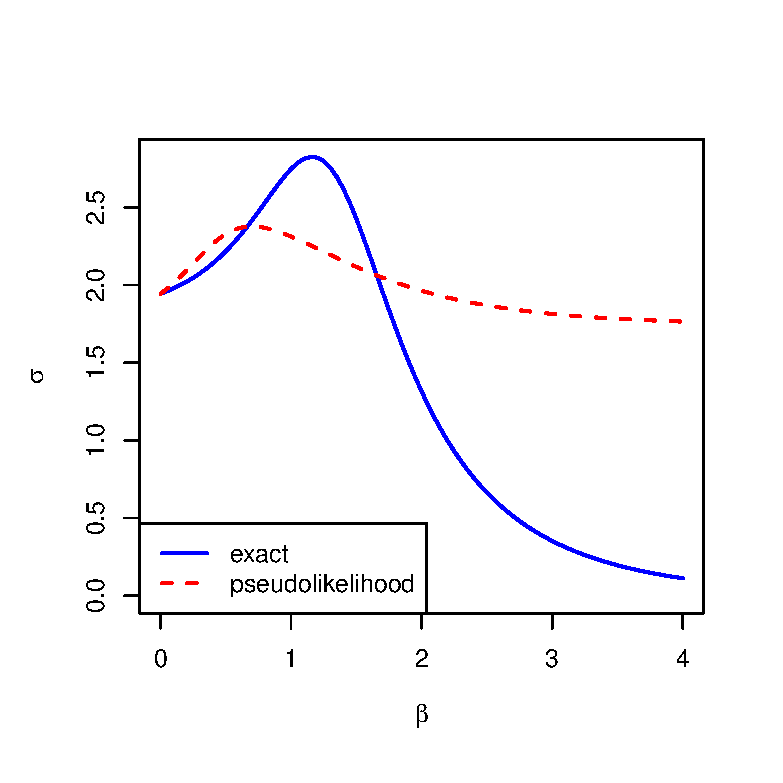
\includegraphics[width=\textwidth]{pl_sd_n12k3.eps}
                \caption{Standard deviation.}
                \label{f:pl_sd}
        \end{subfigure}%
\caption{Approximation error of pseudolikelihood for $n=12,\,k=3$ in comparison to the exact likelihood calculated using a brute force method: (a) $\sum_{\mathbf{z} \in \mathcal{Z}} \mathrm{S}(\mathbf{z}) p(\mathrm{S}(\mathbf{z}) | \beta)$ using either Equation~(\ref{eq:beta}) or (\ref{eq:pseudo}); (b) $\sqrt{\sum_{\mathbf{z} \in \mathcal{Z}} \left( \mathrm{S}(\mathbf{z}) - \mathbb{E}_{\mathbf{z}|\beta}[\mathrm{S}(\mathbf{z})] \right)^2 p(\mathrm{S}(\mathbf{z}) | \beta)}$} 
\label{f:pl}
\end{figure}
Pseudolikelihood is exact when $\beta=0$ and provides a reasonable approximation for small values of the inverse temperature. However, the approximation error increases rapidly for $\beta \ge \beta_{crit}$, as illustrated by Figure~\ref{f:pl}. This is due to long-range dependence between the labels, which is inadequately modelled by the local approximation.

\citet{Ryden1998} referred to Equation~(\ref{eq:pseudo}) in Algorithm~\ref{alg:pseudo} as point pseudolikelihood, since the conditional distributions are computed for each pixel individually. They suggested that the accuracy could be improved using block pseudolikelihood. This is where the likelihood is calculated exactly for small blocks of pixels, then (\ref{eq:pseudo}) is modified to be the product of the blocks:
\begin{equation}
p(\mathbf{z}|\beta) \approx \prod_{i=1}^{N_B} p(\mathbf{z}_{B_i} | \mathbf{z}_{\setminus B_i}, \beta)
\label{eq:pl_comp}
\end{equation}
where $N_B$ is the number of blocks, $\mathbf{z}_{B_i}$ are the labels of the pixels in block $B_i$, and $\mathbf{z}_{\setminus B_i}$ are all of the labels except for $\mathbf{z}_{B_i}$. This is a form of composite likelihood, where the likelihood function is approximated as a product of simplified factors \citep{Varin2011}. \citet{Friel2012} compared point pseudolikelihood to composite likelihood with blocks of $3 \times 3$, $4 \times 4$, $5 \times 5$, and $6 \times 6$ pixels. \citeauthor{Friel2012} showed that (\ref{eq:pl_comp}) outperformed (\ref{eq:pseudo}) for the Ising ($k=2$) model with $\beta < \beta_{crit}$. \citet{Okabayashi2011} discuss composite likelihood for the Potts model with $k > 2$ and have provided an open source implementation in the \proglang{R} package \pkg{potts} \citep{Geyer2014}.

Evaluating the conditional likelihood in (\ref{eq:pl_comp}) involves the normalising constant for $\mathbf{z}_{B_i}$, which is a sum over all of the possible configurations $\mathcal{Z}_{B_i}$. This is a limiting factor on the size of blocks that can be used. The brute force method that was used to compute Figure~\ref{f:exact_beta} and \ref{f:pl} is too computationally intensive for this purpose. \citet{Pettitt2003} showed that the normalising constant can be calculated exactly for a cylindrical lattice by computing eigenvalues of a $k^r \times k^r$ matrix, where $r$ is the smaller of the number of rows or columns. The value of (\ref{eq:norm}) for a free boundary lattice can then be approximated using path sampling. \citet{Friel2004} extended this method to larger lattices using a composite likelihood approach.

The reduced dependence approximation (RDA) is another form of composite likelihood. \citet{Reeves2004} introduced a recursive algorithm to calculate the normalising constant using a lag-$r$ representation. \citet{Friel2009} divided the image lattice into sub-lattices of size $r_1 < r$, then approximated the normalising constant of the full lattice using RDA:
\begin{equation}
\mathcal{C}(\beta) \approx \frac{\mathcal{C}_{r_1 \times n}(\beta)^{r - r_1 + 1}}{\mathcal{C}_{r_1 - 1 \times n}(\beta)^{r - r_1}}
\label{eq:rda}
\end{equation}
\citet{McGrory2009} compared RDA to pseudolikelihood and the exact method of \citet{Moeller2006}, reporting similar computational cost to pseudolikelihood but with improved accuracy in estimating $\beta$. Source code for RDA is available in the online supplementary material for \citet{McGrory2012}.

\subsection{Thermodynamic integration}
\citet{Gelman1998} derived an approximation to the log ratio of normalising constants using the path sampling identity:
\begin{equation}
\label{eq:path}
\log\left\{\frac{\mathcal{C}(\beta_{t-1})}{\mathcal{C}(\beta')}\right\} = \int_{\beta'}^{\beta_{t-1}} \mathbb{E}_{\mathbf{z} | \beta}[\mathrm{S}(\mathbf{z})] \, \mathrm{d}\beta
\end{equation}
which follows from the definition of $\mathbb{E}_{\mathbf{z} | \beta}[\mathrm{S}(\mathbf{z})]$ in (\ref{eq:expSz}). The value of this definite integral can be approximated by simulating from the Gibbs distribution for fixed values of $\beta$ and then interpolating between them. We used the Swendsen-Wang algorithm for simulating from $\mathbf{z}|\beta$, as mentioned in section~\ref{s:model}. Figure~\ref{f:path2d} illustrates linear interpolation of $\mathrm{S}(\mathbf{z})$ on a 2D lattice for $k=6$ and $\beta$ ranging from 0 to 2 in increments of 0.05. This approximation can be precomputed using the same method that was used to produce Figure~\ref{f:bcrit}. Figure~\ref{f:path3d} illustrates interpolation of  $\mathrm{S}(\mathbf{z})$ on a 3D lattice for $k=9$.
\begin{figure}
        \centering
        \begin{subfigure}{0.75\textwidth}
                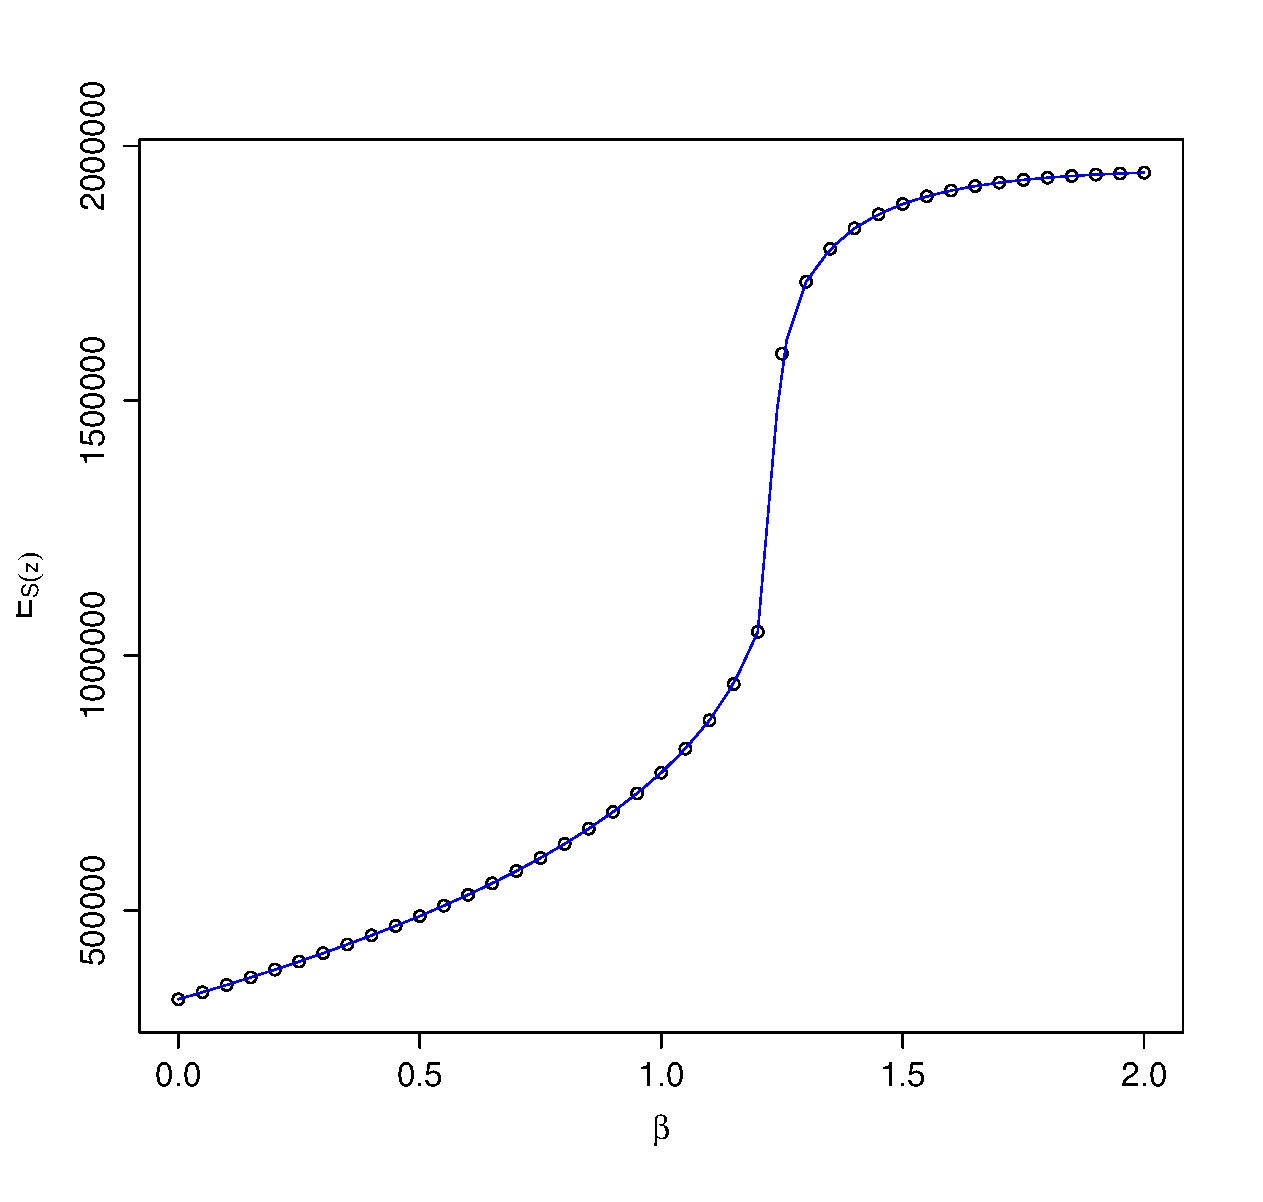
\includegraphics[width=\textwidth]{path2d.eps}
                \caption{2D Potts model with $k=6$.}
                \label{f:path2d}
        \end{subfigure}%
\qquad
        \begin{subfigure}{0.75\textwidth}
                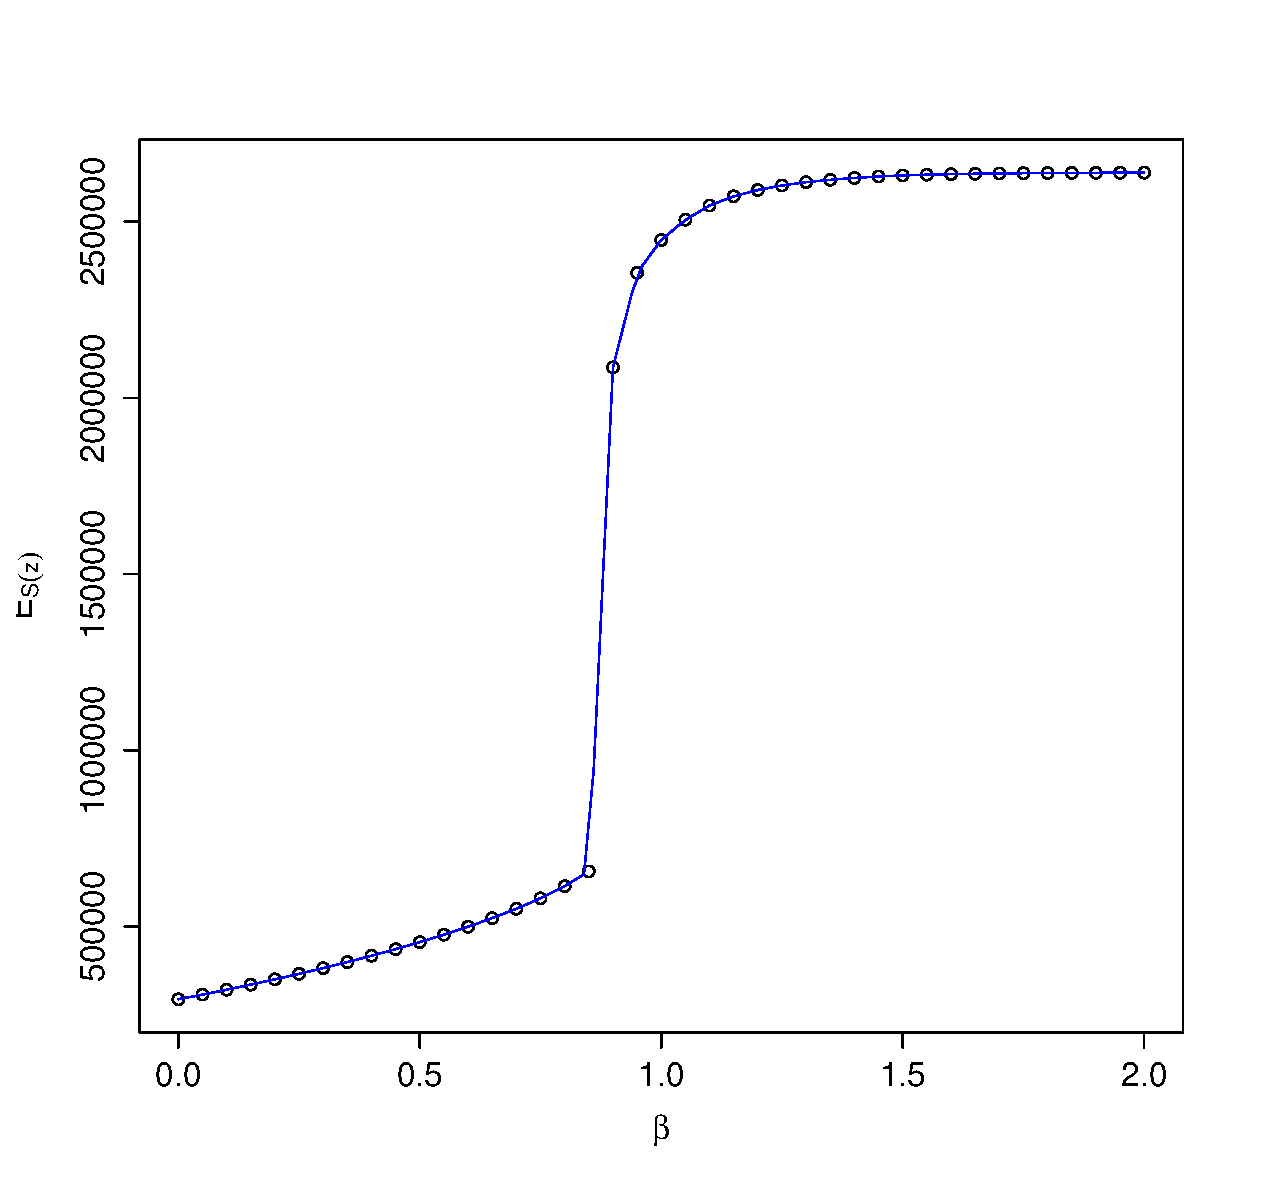
\includegraphics[width=\textwidth]{path3d.eps}
                \caption{3D Potts model with $k=9$.}
                \label{f:path3d}
        \end{subfigure}%
\caption[Approximation of the sufficient statistic by simulation]{Approximation of $\mathbb{E}_{\mathbf{z} | \beta}[\mathrm{S}(\mathbf{z})]$ by simulation for fixed values of $\beta$, with linear interpolation.}
\label{f:path}
\end{figure}


\begin{algorithm}[float,caption={Path sampling (TI)}, label={alg:path}]
Initialise $\beta_0, \boldsymbol\mu_0, \boldsymbol\sigma^2_0, \mathbf{z}_0$
for $t \in 1\dots T$ do
  Update the labels $z_i \sim p(y_i | z_i, \mu_{z_i}, \sigma^2_{z_i}) \,p(z_i | z_{\setminus i}, \beta) \; \forall i \in \{ 1, \dots, n\}$
  Calculate sufficient statistics $\bar{y}_j, s^2_j \; \forall z_i = j, \, \forall j \in \{ 1, \dots, k\}$
  Update the noise parameters $\mu_j, \sigma^2_j \sim p(\bar{y}_j, s^2_j | \mu_j, \sigma_j^2) \,\pi(\mu_j | \sigma^2_j) \, \pi(\sigma^2_j)$
  Draw proposed parameter value $\beta' \sim q(\beta' | \beta_{t-1})$
  Estimate $\mathbb{E}_{\mathbf{z} | \beta}[\mathrm{S}(\mathbf{z})]$ for $\beta \in \{ \beta', \beta_{t-1}\}$ by interpolation
  Evaluate the definite integral in (*@ Equation~\eqref{eq:path} @*)
  Calculate the log M-H acceptance ratio: (*@
  \begin{equation}
  \label{eq:mhRatio_path}
  \log\{\rho\} = \min\left( 0, \log\left\{\frac{\mathcal{C}(\beta_{t-1})}{\mathcal{C}(\beta')}\right\} + (\beta' - \beta_{t-1})\mathrm{S}(\mathbf{z}) + \log\left\{\frac{\pi(\beta') q(\beta_{t-1} | \beta')}{\pi(\beta_{t-1}) q(\beta' | \beta_{t-1})}\right\} \right)
  \end{equation} @*)
  Draw $u \sim \mathrm{Uniform}[0,1]$
  if $u < \rho$ then (*@ \label{mh:accept} @*)
    $\beta_t \gets \beta'$ 
  else
    $\beta_t \gets \beta_{t-1}$ 
  end if
end for
\end{algorithm}

TI is explained in further detail by \citet[chap. 5]{Chen2000}. A reference implementation in R is available from the website accompanying \citet{Marin2007}. This algorithm has an advantage over auxiliary variable methods such as AEA or ABC because the additional simulations are performed prior to fitting the model, rather than at each iteration. This is particularly the case when analysing multiple images that all have approximately the same dimensions. However, the computational cost is still slightly higher than PL, which does not require a pre-computation step.

\subsection{Pseudo-marginal methods}
  \citet{Moeller2006} demonstrated that it is possible to simulate from the posterior distribution of $\beta$ by introducing an auxiliary variable, so that $\mathcal{C}(\beta)$ cancels out in the M-H ratio. The exchange algorithm of \citet{Murray2006} improves the performance of this method and avoids the need for a fixed estimate of $\beta$. The drawback of this approach is that it requires perfect sampling from the stationary distribution of the Potts model. This is possible using coupling from the past \citep{Propp1996,Huber2016} but can be computationally prohibitive, particularly for large images. \citet{McGrory2009} reported that the time required for perfect sampling increased sharply for larger values of $\beta$. For this reason, \citet{Cucala2009} substitute 500 iterations of Gibbs sampling on the auxiliary variable to produce an approximate sample from its stationary distribution. The details of this method are shown in Algorithm~\ref{alg:ex}.
  
\begin{algorithm}[float,caption={Approximate exchange algorithm (AEA)}, label={alg:ex}]
Initialise $\beta_0, \boldsymbol\mu_0, \boldsymbol\sigma^2_0, \mathbf{z}_0$
for $t \in 1\dots T$ do
  Update the labels $z_i \sim p(y_i | z_i, \mu_{z_i}, \sigma^2_{z_i}) \,p(z_i | z_{\setminus i}, \beta) \; \forall i \in \{ 1, \dots, n\}$
  Calculate sufficient statistics $\bar{y}_j, s^2_j \; \forall z_i = j, \, \forall j \in \{ 1, \dots, k\}$
  Update the noise parameters $\mu_j, \sigma^2_j \sim p(\bar{y}_j, s^2_j | \mu_j, \sigma_j^2) \,\pi(\mu_j | \sigma^2_j) \, \pi(\sigma^2_j)$
  Draw proposed parameter value $\beta' \sim q(\beta' | \beta_{t-1})$
  Generate $\mathbf{w}|\beta'$ by sampling from (*@ Equation~(\ref{eq:Potts}) @*)
  Calculate the M-H acceptance ratio according to (*@ Equation~(\ref{eq:beta}): 
  \begin{equation}
  \label{eq:mhRatio_ex}
  \rho =  \min\left( 1, \frac{q(\beta_{t-1}|\beta') \pi(\beta') \exp\left\{ \beta' \mathrm{S}(\mathbf{z}) \right\} \mathcal{C}(\beta_{t-1})}{q(\beta'|\beta_{t-1}) \pi(\beta_{t-1}) \exp\left\{ \beta_{t-1} \mathrm{S}(\mathbf{z}) \right\} \mathcal{C}(\beta')} \frac{\exp\left\{ \beta_{t-1} \mathrm{S}(\mathbf{w}) \right\} \mathcal{C}(\beta')}{\exp\left\{ \beta' \mathrm{S}(\mathbf{w}) \right\} \mathcal{C}(\beta_{t-1})} \right)
  \end{equation} @*)
  Draw $u \sim \mathrm{Uniform}[0,1]$
  if $u < \rho$ then (*@ \label{mh:accept} @*)
    $\beta_t \gets \beta'$ 
  else
    $\beta_t \gets \beta_{t-1}$ 
  end if
end for
\end{algorithm}

The M-H ratio given by Equation~(\ref{eq:mhRatio_ex}) can be considerably simplified if a uniform prior is used for $\beta$ and $\beta'$ is drawn from a symmetric M-H proposal density. In this case, $\log\{\rho\}$ simplifies to $(\beta' - \beta_{t-1})\mathrm{S}(\mathbf{z}) + (\beta_{t-1} - \beta')\mathrm{S}(\mathbf{w})$. The similarity with Equation~(\ref{eq:mhRatio_path}) shows that the exchange algorithm is closely related to path sampling, since it is a form of importance sampling. An implementation of the exchange algorithm is available in the online supplementary material accompanying \citet{Friel2011}. \citet{Everitt2012} provides source code for the approximate exchange algorithm with particle MCMC.

\subsection{Approximate Bayesian computation}
Like the exchange algorithm, ABC uses an auxiliary variable $\mathbf{w}$ to decide whether to accept or reject the proposed value of $\beta'$. Instead of a M-H ratio such as (\ref{eq:mhRatio_ex}), the summary statistics of the auxiliary variable and the observed data are directly compared. The proposal is accepted if the distance between these summary statistics is within the ABC tolerance, $\epsilon$. This produces the following approximation when the labels $\mathbf{z}$ are observed without error:
\begin{equation}
\label{eq:abc_posterior}
p\left(\beta \mid \mathbf{z} \right) \;\approx\; \pi_\epsilon\left(\beta \mid \| \mathrm{S}(\mathbf{w}) - \mathrm{S}(\mathbf{z}) \| < \epsilon\right)
\end{equation}
where $\| \cdot \|$ is a suitable norm. In this paper we simply use the absolute difference between $\mathrm{S}(\mathbf{w})$ and $\mathrm{S}(\mathbf{z})$, since the summary statistic (\ref{eq:potts_stat}) is univariate. $\mathrm{S}(\mathbf{z})$ is sufficient for $\beta$, as noted by \citet{Grelaud2009}, therefore the ABC approximation (\ref{eq:abc_posterior}) approaches the true posterior as $n \to \infty$ and $\epsilon \to 0$. In practice there is a tradeoff between the number of parameter values that are accepted and the size of the ABC tolerance. 

\citet{Everitt2012} introduced ABC for noisy data, such as the Ising model, but only when the observations are discrete and so $\mathrm{S}(\mathbf{y})$ is defined. \citet{Moores2014} showed that ABC can also be applied when the domain of the observed data is continuous, such as with the additive Gaussian noise of Equation~(\ref{eq:obs2}). In this type of model the posterior distribution of $\beta$ does not depend directly on the observed data $\mathbf{y}$, as shown by Equation~(\ref{eq:beta_post}). The ABC approximation (\ref{eq:abc_posterior}) for the hidden Potts model becomes:
\begin{equation}
\label{eq:abc_noise}
p\left(\beta \mid \mathbf{y}, \mathbf{z}, \boldsymbol\theta \right) \;\approx\; \pi_\epsilon\left(\beta \mid \| \mathrm{S}(\mathbf{w}) - \mathrm{S}(\mathbf{z}) \| < \epsilon\right)
\end{equation}
The other parameters can be updated using the current value of $\beta$ and then the summary statistic $\mathrm{S}(\mathbf{z})$ can be computed from the current values of the labels, using an ABC within Gibbs approach as shown in Algorithm~\ref{alg:abc}. Equation~(\ref{eq:abc_noise}) can be considered as a moving target, since $\mathrm{S}(\mathbf{z})$ could change whenever the labels are updated. As a consequence, ABC with noisy data can be more prone to getting stuck in low probability regions of the parameter space.

\citet{Grelaud2009} used a rejection sampler, where the proposals are drawn independently from the prior and thus $q(\beta'|\beta_{t-1}) = \pi(\beta)$. Under a sparse or uninformative prior, such as the uniform prior used in this study, too many proposals are rejected for this approach to be viable. Instead we have based  Algorithm~\ref{alg:abc} on the ABC-MCMC algorithm of \citet{Marjoram2003}. This form of ABC algorithm is best suited for direct comparison with the other intractable likelihood methods in this article.

\begin{algorithm}[float,caption={ABC-MCMC with noisy data}, label={alg:abc}]
Initialise $\beta_0, \boldsymbol\mu_0, \boldsymbol\sigma^2_0, \mathbf{z}_0$
for $t \in 1\dots T$ do
  Update the labels $z_i \sim p(y_i | z_i, \mu_{z_i}, \sigma^2_{z_i}) \,p(z_i | z_{\setminus i}, \beta) \; \forall i \in \{ 1, \dots, n\}$
  Calculate sufficient statistics $\bar{y}_j, s^2_j \; \forall z_i = j, \, \forall j \in \{ 1, \dots, k\}$
  Update the noise parameters $\mu_j, \sigma^2_j \sim p(\bar{y}_j, s^2_j | \mu_j, \sigma_j^2) \,\pi(\mu_j | \sigma^2_j) \, \pi(\sigma^2_j)$
  Draw proposed parameter value $\beta' \sim q(\beta' | \beta_{t-1})$
  Generate $\mathbf{w}|\beta'$ by sampling from (*@ Equation~(\ref{eq:Potts}) @*)
  Draw $u \sim \mathrm{Uniform}[0,1]$
  if $u < \frac{\pi(\beta') q(\beta_{t-1} | \beta')}{\pi(\beta_{t-1}) q(\beta' | \beta_{t-1})}$ and $\| \mathrm{S}(\mathbf{w}) - \mathrm{S}(\mathbf{z}) \| < \epsilon$ then
    $\beta_t \gets \beta'$ 
  else
    $\beta_t \gets \beta_{t-1}$ 
  end if
end for
\end{algorithm}

There have been many extensions to ABC, as reviewed by \citet{Marin2012}. Of particular interest are adaptive ABC algorithms that automatically adjust the tolerance $\epsilon$ and the proposal bandwidth $\sigma^2_{MH}$. ABC with sequential Monte Carlo (SMC-ABC) algorithms use a sequence of target distributions $\pi_{\epsilon_t} \left(\beta \mid \| \mathrm{S}(\mathbf{w}) - \mathrm{S}(\mathbf{z}) \| < \epsilon_t \right)$ such that $\epsilon_1 > \epsilon_2 > \dots > \epsilon_T$, where the number of SMC iterations $T$ can be determined dynamically using a stopping rule. The SMC-ABC algorithm of \citet{Drovandi2011} uses multiple MCMC steps for each SMC iteration, while the algorithm of \citet{DelMoral2012} uses multiple replicates of the summary statistics for each particle. \citet{Everitt2012} has provided a MATLAB implementation of SMC-ABC with the online supplementary material accompanying his paper.

The computational efficiency of ABC is dominated by the cost of drawing updates to the auxiliary variable, as reported by \citet{Everitt2012}. Thus, we would expect that the execution time for ABC would be similar to the approximate exchange algorithm. Various approaches to improving this runtime have recently been proposed, such as the Gaussian process emulation of \citet{Wilkinson2014}, the ``lazy ABC'' of \citet{Prangle2014}, and methods involving auxiliary models \citep{Cabras2014,Moores2014,Buzbas2015}.

\bibliography{InverseTemperature}

\end{document}
